
%% bare_conf.tex
%% V1.4b
%% 2015/08/26
%% by Michael Shell
%% See:
%% http://www.michaelshell.org/
%% for current contact information.
%%
%% This is a skeleton file demonstrating the use of IEEEtran.cls
%% (requires IEEEtran.cls version 1.8b or later) with an IEEE
%% conference paper.
%%
%% Support sites:
%% http://www.michaelshell.org/tex/ieeetran/
%% http://www.ctan.org/pkg/ieeetran
%% and
%% http://www.ieee.org/

%%*************************************************************************
%% Legal Notice:
%% This code is offered as-is without any warranty either expressed or
%% implied; without even the implied warranty of MERCHANTABILITY or
%% FITNESS FOR A PARTICULAR PURPOSE! 
%% User assumes all risk.
%% In no event shall the IEEE or any contributor to this code be liable for
%% any damages or losses, including, but not limited to, incidental,
%% consequential, or any other damages, resulting from the use or misuse
%% of any information contained here.
%%
%% All comments are the opinions of their respective authors and are not
%% necessarily endorsed by the IEEE.
%%
%% This work is distributed under the LaTeX Project Public License (LPPL)
%% ( http://www.latex-project.org/ ) version 1.3, and may be freely used,
%% distributed and modified. A copy of the LPPL, version 1.3, is included
%% in the base LaTeX documentation of all distributions of LaTeX released
%% 2003/12/01 or later.
%% Retain all contribution notices and credits.
%% ** Modified files should be clearly indicated as such, including  **
%% ** renaming them and changing author support contact information. **
%%*************************************************************************


% *** Authors should verify (and, if needed, correct) their LaTeX system  ***
% *** with the testflow diagnostic prior to trusting their LaTeX platform ***
% *** with production work. The IEEE's font choices and paper sizes can   ***
% *** trigger bugs that do not appear when using other class files.       ***                          ***
% The testflow support page is at:
% http://www.michaelshell.org/tex/testflow/



\documentclass[conference]{IEEEtran}
% Some Computer Society conferences also require the compsoc mode option,
% but others use the standard conference format.
%
% If IEEEtran.cls has not been installed into the LaTeX system files,
% manually specify the path to it like:
% \documentclass[conference]{../sty/IEEEtran}





% Some very useful LaTeX packages include:
% (uncomment the ones you want to load)


% *** MISC UTILITY PACKAGES ***
%
%\usepackage{ifpdf}
% Heiko Oberdiek's ifpdf.sty is very useful if you need conditional
% compilation based on whether the output is pdf or dvi.
% usage:
% \ifpdf
%   % pdf code
% \else
%   % dvi code
% \fi
% The latest version of ifpdf.sty can be obtained from:
% http://www.ctan.org/pkg/ifpdf
% Also, note that IEEEtran.cls V1.7 and later provides a builtin
% \ifCLASSINFOpdf conditional that works the same way.
% When switching from latex to pdflatex and vice-versa, the compiler may
% have to be run twice to clear warning/error messages.






% *** CITATION PACKAGES ***
%
%\usepackage{cite}
% cite.sty was written by Donald Arseneau
% V1.6 and later of IEEEtran pre-defines the format of the cite.sty package
% \cite{} output to follow that of the IEEE. Loading the cite package will
% result in citation numbers being automatically sorted and properly
% "compressed/ranged". e.g., [1], [9], [2], [7], [5], [6] without using
% cite.sty will become [1], [2], [5]--[7], [9] using cite.sty. cite.sty's
% \cite will automatically add leading space, if needed. Use cite.sty's
% noadjust option (cite.sty V3.8 and later) if you want to turn this off
% such as if a citation ever needs to be enclosed in parenthesis.
% cite.sty is already installed on most LaTeX systems. Be sure and use
% version 5.0 (2009-03-20) and later if using hyperref.sty.
% The latest version can be obtained at:
% http://www.ctan.org/pkg/cite
% The documentation is contained in the cite.sty file itself.






% *** GRAPHICS RELATED PACKAGES ***
%
\ifCLASSINFOpdf
  \usepackage[pdftex]{graphicx}
  % declare the path(s) where your graphic files are
  % \graphicspath{{../pdf/}{../jpeg/}}
  % and their extensions so you won't have to specify these with
  % every instance of \includegraphics
  % \DeclareGraphicsExtensions{.pdf,.jpeg,.png}
\else
  % or other class option (dvipsone, dvipdf, if not using dvips). graphicx
  % will default to the driver specified in the system graphics.cfg if no
  % driver is specified.
  % \usepackage[dvips]{graphicx}
  % declare the path(s) where your graphic files are
  % \graphicspath{{../eps/}}
  % and their extensions so you won't have to specify these with
  % every instance of \includegraphics
  % \DeclareGraphicsExtensions{.eps}
\fi
% graphicx was written by David Carlisle and Sebastian Rahtz. It is
% required if you want graphics, photos, etc. graphicx.sty is already
% installed on most LaTeX systems. The latest version and documentation
% can be obtained at: 
% http://www.ctan.org/pkg/graphicx
% Another good source of documentation is "Using Imported Graphics in
% LaTeX2e" by Keith Reckdahl which can be found at:
% http://www.ctan.org/pkg/epslatex
%
% latex, and pdflatex in dvi mode, support graphics in encapsulated
% postscript (.eps) format. pdflatex in pdf mode supports graphics
% in .pdf, .jpeg, .png and .mps (metapost) formats. Users should ensure
% that all non-photo figures use a vector format (.eps, .pdf, .mps) and
% not a bitmapped formats (.jpeg, .png). The IEEE frowns on bitmapped formats
% which can result in "jaggedy"/blurry rendering of lines and letters as
% well as large increases in file sizes.
%
% You can find documentation about the pdfTeX application at:
% http://www.tug.org/applications/pdftex





% *** MATH PACKAGES ***
%
%\usepackage{amsmath}
% A popular package from the American Mathematical Society that provides
% many useful and powerful commands for dealing with mathematics.
%
% Note that the amsmath package sets \interdisplaylinepenalty to 10000
% thus preventing page breaks from occurring within multiline equations. Use:
%\interdisplaylinepenalty=2500
% after loading amsmath to restore such page breaks as IEEEtran.cls normally
% does. amsmath.sty is already installed on most LaTeX systems. The latest
% version and documentation can be obtained at:
% http://www.ctan.org/pkg/amsmath





% *** SPECIALIZED LIST PACKAGES ***
%
%\usepackage{algorithmic}
% algorithmic.sty was written by Peter Williams and Rogerio Brito.
% This package provides an algorithmic environment fo describing algorithms.
% You can use the algorithmic environment in-text or within a figure
% environment to provide for a floating algorithm. Do NOT use the algorithm
% floating environment provided by algorithm.sty (by the same authors) or
% algorithm2e.sty (by Christophe Fiorio) as the IEEE does not use dedicated
% algorithm float types and packages that provide these will not provide
% correct IEEE style captions. The latest version and documentation of
% algorithmic.sty can be obtained at:
% http://www.ctan.org/pkg/algorithms
% Also of interest may be the (relatively newer and more customizable)
% algorithmicx.sty package by Szasz Janos:
% http://www.ctan.org/pkg/algorithmicx




% *** ALIGNMENT PACKAGES ***
%
%\usepackage{array}
% Frank Mittelbach's and David Carlisle's array.sty patches and improves
% the standard LaTeX2e array and tabular environments to provide better
% appearance and additional user controls. As the default LaTeX2e table
% generation code is lacking to the point of almost being broken with
% respect to the quality of the end results, all users are strongly
% advised to use an enhanced (at the very least that provided by array.sty)
% set of table tools. array.sty is already installed on most systems. The
% latest version and documentation can be obtained at:
% http://www.ctan.org/pkg/array


% IEEEtran contains the IEEEeqnarray family of commands that can be used to
% generate multiline equations as well as matrices, tables, etc., of high
% quality.




% *** SUBFIGURE PACKAGES ***
%\ifCLASSOPTIONcompsoc
%  \usepackage[caption=false,font=normalsize,labelfont=sf,textfont=sf]{subfig}
%\else
%  \usepackage[caption=false,font=footnotesize]{subfig}
%\fi
% subfig.sty, written by Steven Douglas Cochran, is the modern replacement
% for subfigure.sty, the latter of which is no longer maintained and is
% incompatible with some LaTeX packages including fixltx2e. However,
% subfig.sty requires and automatically loads Axel Sommerfeldt's caption.sty
% which will override IEEEtran.cls' handling of captions and this will result
% in non-IEEE style figure/table captions. To prevent this problem, be sure
% and invoke subfig.sty's "caption=false" package option (available since
% subfig.sty version 1.3, 2005/06/28) as this is will preserve IEEEtran.cls
% handling of captions.
% Note that the Computer Society format requires a larger sans serif font
% than the serif footnote size font used in traditional IEEE formatting
% and thus the need to invoke different subfig.sty package options depending
% on whether compsoc mode has been enabled.
%
% The latest version and documentation of subfig.sty can be obtained at:
% http://www.ctan.org/pkg/subfig




% *** FLOAT PACKAGES ***
%
%\usepackage{fixltx2e}
% fixltx2e, the successor to the earlier fix2col.sty, was written by
% Frank Mittelbach and David Carlisle. This package corrects a few problems
% in the LaTeX2e kernel, the most notable of which is that in current
% LaTeX2e releases, the ordering of single and double column floats is not
% guaranteed to be preserved. Thus, an unpatched LaTeX2e can allow a
% single column figure to be placed prior to an earlier double column
% figure.
% Be aware that LaTeX2e kernels dated 2015 and later have fixltx2e.sty's
% corrections already built into the system in which case a warning will
% be issued if an attempt is made to load fixltx2e.sty as it is no longer
% needed.
% The latest version and documentation can be found at:
% http://www.ctan.org/pkg/fixltx2e


%\usepackage{stfloats}
% stfloats.sty was written by Sigitas Tolusis. This package gives LaTeX2e
% the ability to do double column floats at the bottom of the page as well
% as the top. (e.g., "\begin{figure*}[!b]" is not normally possible in
% LaTeX2e). It also provides a command:
%\fnbelowfloat
% to enable the placement of footnotes below bottom floats (the standard
% LaTeX2e kernel puts them above bottom floats). This is an invasive package
% which rewrites many portions of the LaTeX2e float routines. It may not work
% with other packages that modify the LaTeX2e float routines. The latest
% version and documentation can be obtained at:
% http://www.ctan.org/pkg/stfloats
% Do not use the stfloats baselinefloat ability as the IEEE does not allow
% \baselineskip to stretch. Authors submitting work to the IEEE should note
% that the IEEE rarely uses double column equations and that authors should try
% to avoid such use. Do not be tempted to use the cuted.sty or midfloat.sty
% packages (also by Sigitas Tolusis) as the IEEE does not format its papers in
% such ways.
% Do not attempt to use stfloats with fixltx2e as they are incompatible.
% Instead, use Morten Hogholm'a dblfloatfix which combines the features
% of both fixltx2e and stfloats:
%
% \usepackage{dblfloatfix}
% The latest version can be found at:
% http://www.ctan.org/pkg/dblfloatfix




% *** PDF, URL AND HYPERLINK PACKAGES ***
%
%\usepackage{url}
% url.sty was written by Donald Arseneau. It provides better support for
% handling and breaking URLs. url.sty is already installed on most LaTeX
% systems. The latest version and documentation can be obtained at:
% http://www.ctan.org/pkg/url
% Basically, \url{my_url_here}.




% *** Do not adjust lengths that control margins, column widths, etc. ***
% *** Do not use packages that alter fonts (such as pslatex).         ***
% There should be no need to do such things with IEEEtran.cls V1.6 and later.
% (Unless specifically asked to do so by the journal or conference you plan
% to submit to, of course. )


% correct bad hyphenation here
\hyphenation{op-tical net-works semi-conduc-tor}


\begin{document}
%
% paper title
% Titles are generally capitalized except for words such as a, an, and, as,
% at, but, by, for, in, nor, of, on, or, the, to and up, which are usually
% not capitalized unless they are the first or last word of the title.
% Linebreaks \\ can be used within to get better formatting as desired.
% Do not put math or special symbols in the title.
\title{Multi-Stage Ensemble and Feature Engineering for MOOC Dropout Prediction}


% author names and affiliations
% use a multiple column layout for up to three different
% affiliations
\author{\IEEEauthorblockN{Anonymous}
\IEEEauthorblockA{Anonymous\\
anonymous@anonymous.com}
\and
\IEEEauthorblockN{Anonymous}
\IEEEauthorblockA{Anonymous\\
anonymous@anonymous.com}
\and
\IEEEauthorblockN{Anonymous}
\IEEEauthorblockA{Anonymous\\
anonymous@anonymous.com}
}

% conference papers do not typically use \thanks and this command
% is locked out in conference mode. If really needed, such as for
% the acknowledgment of grants, issue a \IEEEoverridecommandlockouts
% after \documentclass

% for over three affiliations, or if they all won't fit within the width
% of the page, use this alternative format:
% 
%\author{\IEEEauthorblockN{Michael Shell\IEEEauthorrefmark{1},
%Homer Simpson\IEEEauthorrefmark{2},
%James Kirk\IEEEauthorrefmark{3}, 
%Montgomery Scott\IEEEauthorrefmark{3} and
%Eldon Tyrell\IEEEauthorrefmark{4}}
%\IEEEauthorblockA{\IEEEauthorrefmark{1}School of Electrical and Computer Engineering\\
%Georgia Institute of Technology,
%Atlanta, Georgia 30332--0250\\ Email: see http://www.michaelshell.org/contact.html}
%\IEEEauthorblockA{\IEEEauthorrefmark{2}Twentieth Century Fox, Springfield, USA\\
%Email: homer@thesimpsons.com}
%\IEEEauthorblockA{\IEEEauthorrefmark{3}Starfleet Academy, San Francisco, California 96678-2391\\
%Telephone: (800) 555--1212, Fax: (888) 555--1212}
%\IEEEauthorblockA{\IEEEauthorrefmark{4}Tyrell Inc., 123 Replicant Street, Los Angeles, California 90210--4321}}




% use for special paper notices
%\IEEEspecialpapernotice{(Invited Paper)}




% make the title area
\maketitle

% As a general rule, do not put math, special symbols or citations
% in the abstract
\begin{abstract}
In this paper, we present the winning solution of KDD Cup 2015, where participants are asked to predict dropouts in a Massive Open Online Course (MOOC) platform.  
Our approach demonstrates best practices in feature engineering dealing with complex real world data, and pushes forward state-of-the-art for ensemble methods.
We began with feature engineering.  We extracted the hand-crafted and autoencoder features from raw student activity logs, course enrollment, and course material data.  
Then, we trained 64 classifiers with 8 different algorithms and different subsets of extracted features.  Lastly, we blended predictions of classifiers with the multi-stage ensemble framework.  
Our final solution achieved AUC scores of 0.90918 and 0.90744 on the public and private leaderboards respectively, and put us to the 1st place out of 821 teams.
\end{abstract}

% no keywords




% For peer review papers, you can put extra information on the cover
% page as needed:
% \ifCLASSOPTIONpeerreview
% \begin{center} \bfseries EDICS Category: 3-BBND \end{center}
% \fi
%
% For peerreview papers, this IEEEtran command inserts a page break and
% creates the second title. It will be ignored for other modes.
\IEEEpeerreviewmaketitle



\section{Introduction}
The task of KDD Cup 2015 is to predict the likelihood of dropout for students on XuetangX, one of the largest Massive Open Online Course (MOOC) platforms in China.

Activity logs of 200,906 enrollments from 112,448 students across 39 courses are provided.
Each activity is described by 6 fields of the username, course ID, timestamp, source, event, and object. 
For each object, 3 additional fields of the category, children, and start date are provided.
The training set consists of 8,157,278 logs from 120,543 enrollments with the target variable indicating if a student dropped out.  
The test set consists of 5,387,848 logs from 80,363 enrollments.
The full description of the data sets is available in \cite{kddcup2015_data}



Our final solution is a joint work from 9 data scientists, distributed around the world.
The pipeline from raw data to final solution is as follows:
\begin{itemize}
  \setlength\itemsep{0em}
  \item Hand crafted feature engineering (most of hard work)
  \item Automatic feature design (autoencoder)
  \item Individual models (gbm, nn, factor model,..)
  \item Stage-I ensemble (blends individual models)
  \item Stage-II ensemble (blends stage-I ensemble models)
  \item Stage-III ensemble (blends stage-II ensemble models)
\end{itemize}

% I think our ensemble framework is different from Otto competition winner's:  Theirs is a stage-II and ours is a stage-III.
% This approach was published by a winning team of Otto kaggle competition \cite{otto},\cite{triskelion}.
\section{Feature Engineering}
Our team members extracted 7 feature sets, namely F1, F2, F3, F4, F5, F6, and F7 from raw data independently.

\subsection{Data Sets}
Activity logs of 200,906 enrollments from 112,448 students across 39 courses are provided.
Each activity is described by 6 fields of the username, course ID, timestamp, source, event, and object. 
For each object, 3 additional fields of the category, children, and start date are provided.
The training set consists of 8,157,278 logs from 120,543 enrollments with the target variable indicating if a student dropped out.  
The test set consists of 5,387,848 logs from 80,363 enrollments.
The full description of the data sets is available in \cite{kddcup2015_data}. In general, this data can be organized in three dimension space, object, time, and event as shown in Figure~\ref{fig:cube}. Feature engineering tasks were carried out based on these views.

\begin{figure*}[!t]
	\caption{Data Cube}
	\centering
	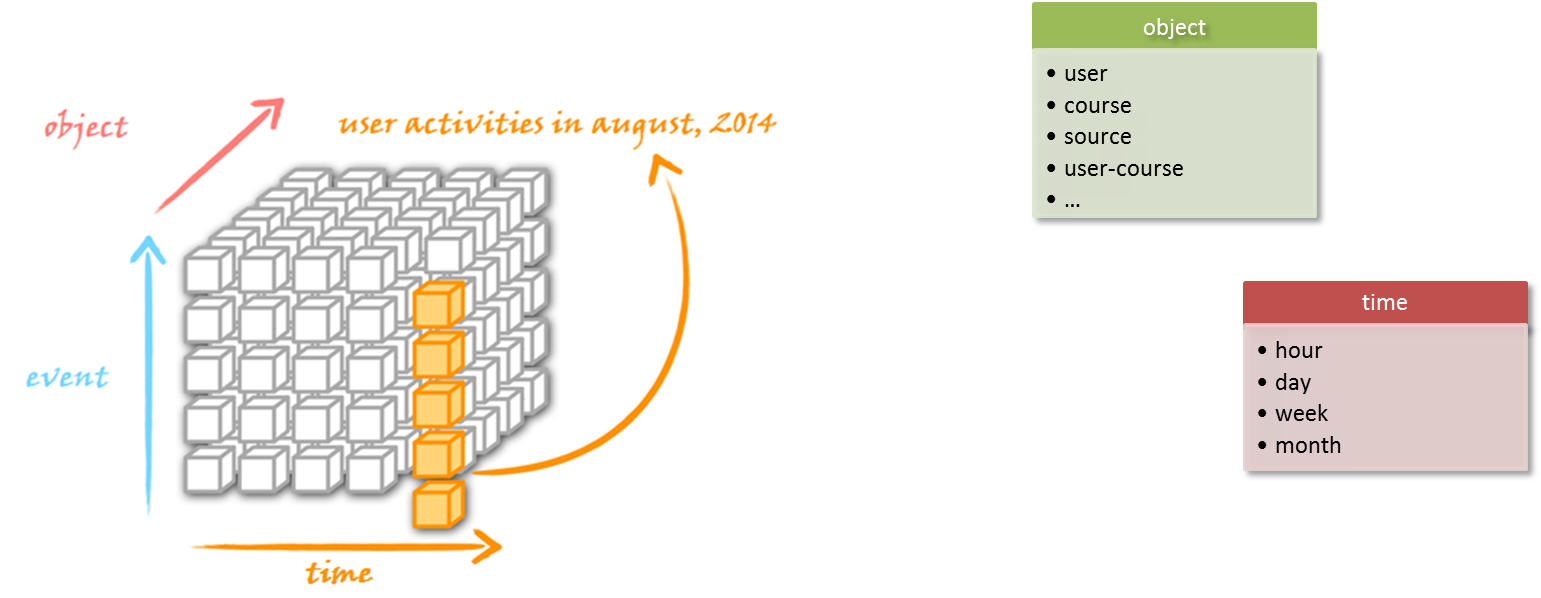
\includegraphics[width=1 \textwidth]{cube}
	\label{fig:cube}
\end{figure*}


\subsection{Common Features}
There are common features across 7 feature sets as follows:
\begin{itemize}
	\item Number of objects
	\item Number of events
	\item Aggregation features these count features
\end{itemize}
The common features can be generated using cube operations. Figure~\ref{fig:slice} shows an example how weekly and monthly count features are calculated. Firstly, the data is cut using object dimension. In this case, we choose to generate feature for users. Next, we select an event "navigate" in the event space to generate a time series presenting "navigate" event over the time. Finally, drill down operation is used to generate monthly or weekly count features.

\begin{figure*}[!t]
	\caption{Slice and Dice}
	\centering
	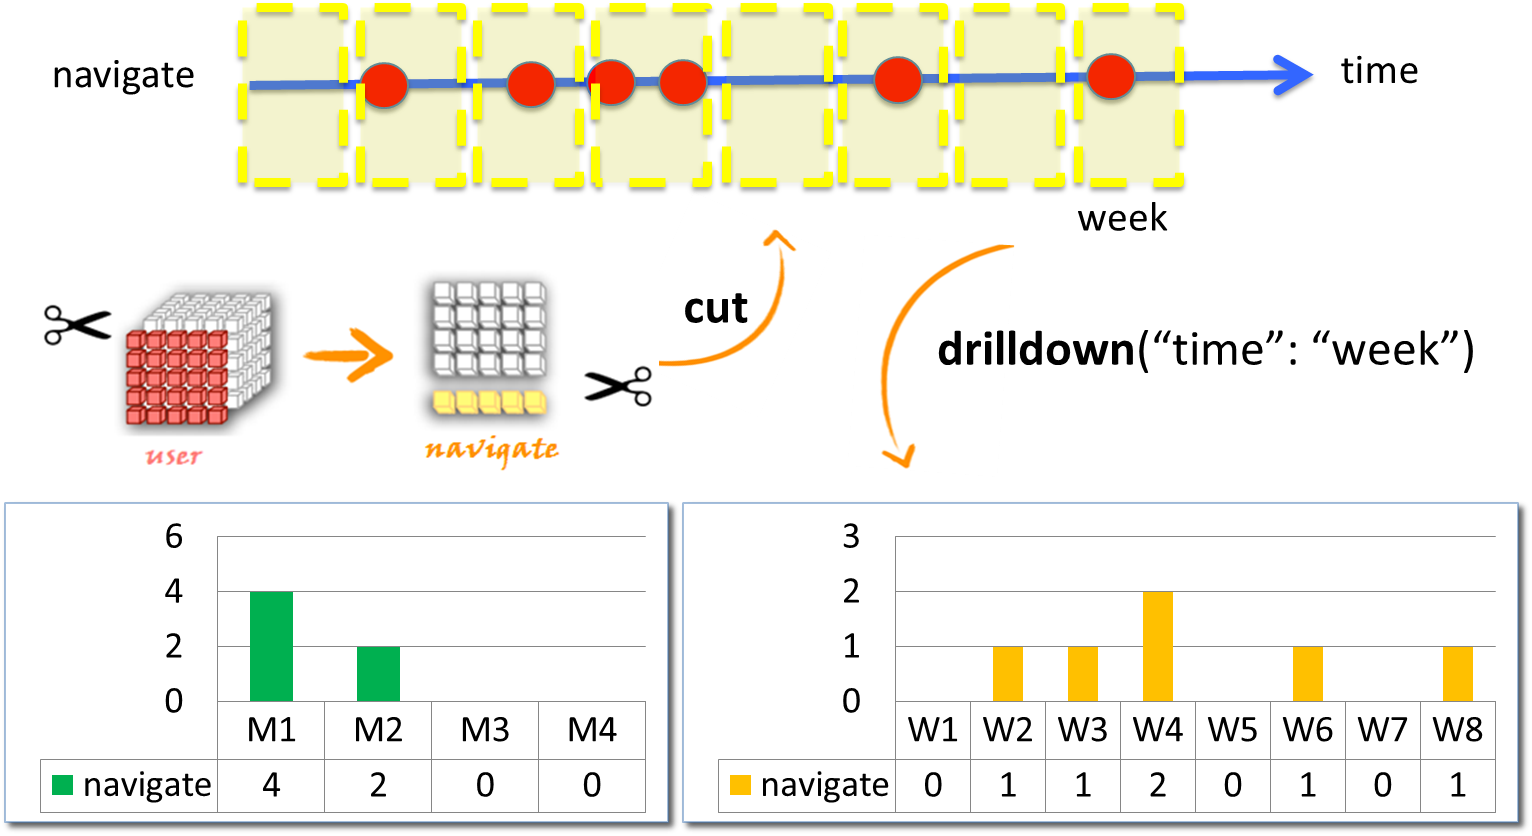
\includegraphics[width=1 \textwidth]{slice_and_dice}
	\label{fig:slice}
\end{figure*}

\subsection{F1}

Features generated by Song and Kohei can be classified as follows:

\begin{itemize}
  \setlength\itemsep{0em}
  \item Enrollment-based features (No.1-8)
  \item Username-based features (No.9-18)
  \item Username-based features for each courses (No.19-25) 
  \item Features based on 10 days after the end date of course (No.26-35)
  \item Features based on 1 day after the end date of a course (No.36-45)
  \item Day-level features (No.46)
  \item Day-level features using target variables (No.47-58)
\end{itemize}

Full list of features generated by Song and Kohei are described in Table~\ref{tb:skfeature}.
(just listing them for now. TBD in detail).

\begin{center}
  \begin{table*}[ht]
    \begin{minipage}{\textwidth}
    {
      \small
      \hfill{}
      \begin{tabular}{|l|l|}
      \hline
      \textbf{No.}&\textbf{Description}\tabularnewline \hline
      1 & Course\_id encoded by 1-of-N coding \tabularnewline
      2 & Number of requests by an enrollment\_id \tabularnewline
      3 & Number of unique object by an enrollment\_id \tabularnewline
      4 & Number of unique problem object of event by an enrollment\_id \tabularnewline
      5 & Number of active days by an enrollment\_id \tabularnewline
      6 & Number of active hours by an enrollment\_id \tabularnewline
      7 & Time of first access in hours by an enrollment\_id \tabularnewline
      8 & Time of last access in hours by an enrollment\_id \tabularnewline
      9 & Number of enrollments by an username \tabularnewline
      10 & Number of requests by an username \tabularnewline
      11 & Number of unique objects by an username \tabularnewline
      12 & Number of unique problem object of event by an username \tabularnewline
      13 & Number of active days by an username \tabularnewline
      14 & Number of active hours by an username \tabularnewline
      15 & Time of first access in hours by an username \tabularnewline
      16 & Time of last access in hours by an username \tabularnewline
      17 & Time of first problem access in hours by an username \tabularnewline
      18 & Time of last problem access in hours by an username \tabularnewline
      19 & For each course, number of requests by an username \tabularnewline
      20 & For each course, number of unique object by an username \tabularnewline
      21 & For each course, number of unique problem object by an username \tabularnewline
      22 & For each course, number of active days by an username \tabularnewline
      23 & For each course, number of active hours by an username \tabularnewline
      24 & For each course, time of first access in hours \tabularnewline
      25 & For each course, time of last access in hours \tabularnewline
      26 & Number of enrollment\_ids during 10 days after the end date of course by an username \tabularnewline
      27 & For each course, number of access logs during 10 days after the end date of course by an username \tabularnewline
      28 & For each course, number of unique objects during 10 days after the end date of course by an username \tabularnewline
      29 & For each course, number of unique problem objects during 10 days after the end date of course by an username \tabularnewline
      30 & For each course, number of active hours during 10 days after the end date of course by an username \tabularnewline
      31 & For each course, difference between first and last access during 10 days after the end date of course by an username \tabularnewline
      32 & For each course, time of first access in hours during 10 days after the end date of course by an username \tabularnewline
      33 & For each course, time of last access in hours during 10 days after the end date of course by an username \tabularnewline
      34 & For each course, time of first access to an problem object in hours during 10 days after the end date of course by an username \tabularnewline
      35 & For each course, time of last access to an problem object in hours during 10 days after the end date of course by an username \tabularnewline
      36 & Number of enrollment\_ids during 1 day after the end date of course by an username \tabularnewline
      37 & For each course, number of access logs during 1 day after the end date of course by an username \tabularnewline
      38 & For each course, number of unique objects during 1 day after the end date of course by an username \tabularnewline
      39 & For each course, number of unique problem objects during 1 day after the end date of course by an username \tabularnewline
      40 & For each course, number of active hours during 1 day after the end date of course by an username \tabularnewline
      41 & For each course, difference between first and last access during 1 day after the end date of course by an username \tabularnewline
      42 & For each course, time of first access in hours during 1 day after the end date of course by an username \tabularnewline
      43 & For each course, time of last access in hours during 1 day after the end date of course by an username \tabularnewline
      44 & For each course, time of first access to an problem object in hours during 1 day after the end date of course by an username \tabularnewline
      45 & For each course, time of last access to an problem object in hours during 1 day after the end date of course by an username \tabularnewline
      46 & For each days of the course, which date is provided in date.csv, number of unique active courses by an username \tabularnewline
      \hline
      \end{tabular}
    }
    \hfill{}
    \caption{List of features generated by Song and Kohei.}
    \label{tb:skfeature}
    \end{minipage}
  \end{table*}
\end{center}

\subsection{F2}
Peng and Xiaocong features are comprised of the following parts:
\begin{itemize}
  \setlength\itemsep{0em}
  \item Visit time(hour, day) set features (including time span and max absent days)
  \item Act(event, object) counting features (some uses missed content counts)
  \item Course drop rate
  \item Number of courses the user enrolled
  \item Minimum time interval between time points(first visit, last visit, course begin, course end, 10 days after course end) of current course and another enrolled course
  \item Active days between course end and 10 days after course end
  \item Active days between last visit and course end
  \item Number of courses ended after current course end
\end{itemize}

The full feature list could be found in Table~\ref{tb:rwfeature}.

\begin{center}
  \begin{table*}[ht]
    \begin{minipage}{\textwidth}
    {
      \small
      \hfill{}
      \begin{tabular}{|l|l|}
      \hline
      \textbf{No.}&\textbf{Description}\tabularnewline \hline
1 & act counts \tabularnewline
2 & hourset length in last 2 days \tabularnewline
3 & last month \tabularnewline
4 & max absent days \tabularnewline
5 & day set length \tabularnewline
6 & hour set length \tabularnewline
7 & average hours per day \tabularnewline
8 & event wiki counts \tabularnewline
9 & event discussion counts \tabularnewline
10 & event access counts \tabularnewline
11 & event video counts \tabularnewline
12 & event problem counts \tabularnewline
13 & obj chapter not visited \tabularnewline
14 & obj chapter visited ratio \tabularnewline
15 & obj video not visited \tabularnewline
16 & obj video visited ratio \tabularnewline
17 & obj problem not visited \tabularnewline
18 & obj problem visited ratio \tabularnewline
19 & obj set length \tabularnewline
20 & total time span \tabularnewline
21 & days from last act to course end \tabularnewline
22 & course drop rate \tabularnewline
23 & number of courses enrolled \tabularnewline
24 & min days between first visit and next course begin \tabularnewline
25 & min days between 10 days after last visit and next course begin \tabularnewline
26 & min days between last visit and next course end \tabularnewline
27 & min days between previous course end and last visit \tabularnewline
28 & min days between 10 days after current course end and next course begin \tabularnewline
29 & min days between 10 days after current course end and next course end \tabularnewline
30 & min days between current course end and next visit \tabularnewline
31 & number of active days between last visit and course end \tabularnewline
32 & number of active days in 10 days after course end \tabularnewline
33 & number of courses ended after current course end \tabularnewline
      \hline
      \end{tabular}
    }
    \hfill{}
    \caption{List of features generated by Peng and Xiaocong.}
    \label{tb:rwfeature}
    \end{minipage}
  \end{table*}
\end{center}

\subsection{F3}
These features were generated by Tam. They can be categorized into three major groups, count, aggregation, and date features. The list of features is as follows:
\subsubsection{Count Feature}
There are a few entities such as user, course, and object in the training dataset. Combining these entities together, we have user activities or events. The simplest way to generate features from these events is to count the number of times an entity engaging in the event. The motivation is that the more does a user participate in course, the more chance does he drop out that course. The list of count features are given in Table~\ref{tb:tnfeature1}.

\begin{center}
	\begin{table*}[ht]
		\begin{minipage}{\textwidth}
			{
				\small
				\hfill{}
				\begin{tabular}{|l|l|l|}
					\hline
					\textbf{No.}&\textbf{Feature}&\textbf{Description}\tabularnewline \hline
					1 & User counts & The log count of each user \tabularnewline
					2 & Course count & The log count of each course \tabularnewline
					3 & Event count & The log count of each event \tabularnewline
					4 & User weekly count & The log count of each user per week \tabularnewline
					5 & User bi-weekly count & The log count of each user per two weeks \tabularnewline
					6 & User weekday count & The log count of each user per weekday \tabularnewline
					7 & User monthly count & The log count of each user per month\tabularnewline
					8 & Course weekly count & The log count of each course per week \tabularnewline
					9 & Course bi-weekly count & The log count of each course per two weeks \tabularnewline
					10 & Course weekday count & The log count of each course per weekday\tabularnewline
					11 & Course monthly count & The log count of each course per month \tabularnewline
					12 & Event weekly count & The log count of each event per week \tabularnewline
					13 & Event bi-weekly count & The log count of each event per two weeks \tabularnewline
					14 & Event weekday count & The log count of each event per weekday \tabularnewline
					15 & Event monthly count & The log count of each event per month \tabularnewline
					\hline
				\end{tabular}
			}
			\hfill{}
			\caption{List of count features generated by Tam.}
			\label{tb:tnfeature1}
		\end{minipage}
	\end{table*}
\end{center}

\subsubsection{Aggregation Feature}
Aggregation features were calculated based on count features. Usually, each course would have a fixed schedule for users to study. Therefore, students roll in the course must have stable activity patterns. Aggregation features would measure the stability of course engagement. These features are mean, median, standard deviation of count on date basis such as weekly, monthly, etc. The list of aggregation features are given in Table~\ref{tb:tnfeature2}.

\begin{center}
	\begin{table*}[ht]
		\begin{minipage}{\textwidth}
			{
				\small
				\hfill{}
				\begin{tabular}{|l|l|l|}
					\hline
					\textbf{No.}&\textbf{Feature}&\textbf{Description}\tabularnewline \hline
					1 & Min & Min of all above count features \tabularnewline
					2 & Max & Max of all above count features \tabularnewline
					3 & Mean & Mean of all above count features \tabularnewline
					4 & Median & Median of all above count features \tabularnewline
					5 & Std & Standard deviation of all above count features  \tabularnewline
					\hline
				\end{tabular}
			}
			\hfill{}
			\caption{List of aggregation features generated by Tam.}
			\label{tb:tnfeature2}
		\end{minipage}
	\end{table*}
\end{center}

\subsubsection{Date Feature}
To capture how often users participate in a certain course, we generated date features. Date features can be time span among user activities as well as time span from last activity and last course date. The list of date features is given in Table~\ref{tb:tnfeature3}.

\begin{center}
	\begin{table*}[ht]
		\begin{minipage}{\textwidth}
			{
				\small
				\hfill{}
				\begin{tabular}{|l|l|l|}
					\hline
					\textbf{No.}&\textbf{Feature}&\textbf{Description}\tabularnewline \hline
					1 & Min time span & Min time span among activities \tabularnewline
					2 & Max time span & Max time span among activities \tabularnewline
					3 & Mean time span & Mean time span among activities \tabularnewline
					4 & Last time span & Time span from the last activity and last course date \tabularnewline
					5 & Number of unique days & The number of unique activity days of each user \tabularnewline
					\hline
				\end{tabular}
			}
			\hfill{}
			\caption{List of date features generated by Tam.}
			\label{tb:tnfeature3}
		\end{minipage}
	\end{table*}
\end{center}

\subsection{F4}
Features generated by Michael Jahrer are in sparse format:

\begin{itemize}
  \setlength\itemsep{0em}
  \item uID (0-112,447)
  \item cID (112,448-112,486)
  \item uIDcnt (112,487-112,487)
  \item eIDcnt (112,488-112,488)
  \item eID $\rightarrow$ sID (112,489-112,490)
  \item eID $\rightarrow$ evID (11,2491-112,497)
  \item eID $\rightarrow$ oIDCnt (112,498-139,443)
  \item eID $\rightarrow$ tIDCnt (139,444-139,635)
  \item uID: floor(log(dateSpan$^2$+1)) (139,636-140,635)
  \item uID $\rightarrow$ log(time diff to obj start+1) (140,636-140,636)
  \item eID $\rightarrow$ dateVec diff stats (140,637-140,649)
\end{itemize}

\subsection{F5}
\begin{itemize}
  \setlength\itemsep{0em}
  \item Course ID - One-hot-encoded course\_id
  \item Source time counts  by enrollment - The log count of each source type per day for each enrollment
  \item Source time counts by course id - The log count of each source type per day for each course id
  \item Event time counts by enrollment - The log count of each event type per day for each enrollment
  \item Event time counts by course id - The log count of each event type per day for each course id

\end{itemize}

\subsection{F6}
Features generated by Jeong-Yoon Lee are as follows:

\begin{itemize}
  \setlength\itemsep{0em}
  \item User ID (20,113) - One-hot-encoded username. Usernames appearing less than 100 times in training log data are grouped together as one user ID. 
  \item Course ID (39) - One-hot-encoded course\_id.
  \item Source Event (10) - One-hot-encoded combination of source and event.
  \item Object ID (3,554) - One-hot-encoded object.  Objects appearing less than 100 times in training log data are grouped together as one object ID.
  \item Count (1) - Number of log entries for an hour\_id.
  \item Object Category (6) - Number of log entries with an object category for an enrollment\_id.
  \item Number of Children Objects (7) - One-hot-encoded total number of object's children for an enrollment\_id.
  \item Object Timespan (10) - One-hot-encoded timespan in days between object's start date and last day of the class
  \item Day of Class (30) - One-hot-encoded day of the class
  \item Week of Class (4) - One-hot-encoded week of the class
  \item End Month of Class (7) - One-hot-encoded end month of the class
  \item Object Started in Dropout Period (2) - Binary variable that is 1 if object started after but before 10 days after last day of the class and 0 otherwise.
\end{itemize}

\subsection{F7}

F1 features and additional features generated by Kohei. Additional features are as follows:

\begin{center}
  \begin{table*}[ht]
    \begin{minipage}{\textwidth}
    {
      \small
      \hfill{}
      \begin{tabular}{|l|l|}
      \hline
      \textbf{No.}&\textbf{Description}\tabularnewline \hline
      1 & For each 10 days after the end date of the course, number of active enrollment\_id, which target variables are 1 in the training set, enrolled by an username \tabularnewline 
      2 & For each 10 days after the end date of the course, number of active enrollment\_id, which target variables are 0 in the training set, enrolled by an username \tabularnewline 
      3 & For each 10 days after the end date of the course, number of active enrollment\_id (in this case, days between last access and the end date of the course are also counted for active days), which target variables are 1 in the training set, enrolled by an username \tabularnewline
      4 & For each 10 days after the end date of the course, number of active enrollment\_id (in this case, days between last access and the end date of the course are also counted for active days), which target variables are 0 in the training set, enrolled by an username \tabularnewline
      5 & For each 14 days before the end date of the coruses, number of active enrollment\_id, which target variables are 1 in the training set, enrolled by an username \tabularnewline 
      6 & For each 14 days before the end date of the coruses, number of active enrollment\_id, which target variables are 0 in the training set, enrolled by an username \tabularnewline 
      7 & For each 14 days before the end date of the coruses, number of active enrollment\_id (in this case, days between last access and the end date of the course are also counted for active days), which target variables are 1 in the training set, enrolled by an username \tabularnewline
      8 & For each 14 days before the end date of the coruses, number of active enrollment\_id (in this case, days between last access and the end date of the course are also counted for active days), which target variables are 0 in the training set, enrolled by an username \tabularnewline
      \hline
      \end{tabular}
    }
    \hfill{}
    \caption{List of additional features generated by Kohei.}
    \label{tb:skfeature}
    \end{minipage}
  \end{table*}
\end{center}

\section{Classification Algorithms}
We selected algorithms that achieve good predictive performance, process large sparse data sets efficiently (with exception of K-Nearest Neighbors) and differ from other algorithms.  The 8 classification algorithms selected are as follows:
\begin{itemize}
\setlength\itemsep{0em}
\item \textbf{Gradient Boosting Machine (GBM)}: We trained GBM classifiers using the Scikit-Learn Python package \cite{scikit-learn} and XGBoost \cite{chen2015xgboost}.  We used various tree structures of 4 to 10 maximum depths and 0.004 to 0.05 shrinkage rates.
\item \textbf{Neural Networks (NN)}: We trained NN classifiers with the dropout \cite{srivastava2014dropout}, ReLU transfer function and sigmoid activation function.  We used various network architectures of 1 to 3 hidden layers and 16 to 500 hidden units per layer.  We wrote our own C++ NN implementation optimized for sparse data sets.  
\item \textbf{Factorization Machine (FM)}: We trained FM classifiers using libFM \cite{rendle2012factorization} and libFFM \cite{libffm}.  We used 2-way interaction dimensions of 4 to 20.  We transformed count variables $x$ into $\log{(1 + x)}$.
\item \textbf{Logistic Regression (LR)}: We trained LR classifiers using the Scikit-Learn Python package \cite{scikit-learn} and Vowpal Wabbit \cite{langford2007vowpal}.  We used the regularization parameter $C=0.01$.  We transformed count variables $x$ into $\log{(1 + x)}$.
\item \textbf{Kernel Ridge Regression (KRR)}: We trained KRR classifiers using our own C++ implementation.  We used the ridge regression constant $\lambda=1.5e-3$ with the Gaussian kernel.  We transformed count variables $x$ into $\log{(1 + x)}$.
\item \textbf{Extremely Randomized Trees (ET)}: We trained ET classifiers using the Scikit-Learn Python package \cite{scikit-learn}.
\item \textbf{Random Forests (RF)}: We trained RF classifiers using the Scikit-Learn Python package \cite{scikit-learn}.  Besides training classifiers, we used RF for feature selection.  We trained an RF model and selected features with high variable importances.
\item \textbf{K-Nearest Neighbors (KNN)}: We trained KNN classifiers using our own C++ implementation.  We used $k=124$ with the Euclidean distance.  We transformed count variables $x$ into $\log{(1 + x)}$.
\end{itemize}
\section{Learning Framework}
At previous KDD Cups, winning solutions either combined only single models without further combining ensemble models \cite{guyon2009analysis, yu2010feature} or combined ensemble models based on public leaderboard scores, which are not available in practice \cite{chen2011, wu2012two}.

However, we were able to combine ensemble models in multiple stages without overfitting to training data or using public leaderboard scores by using our learning framework.  Our learning framework consists of the stratified cross validation (CV) and multi-stage ensemble.

\subsection{Model Validation}

\begin{figure}
  \centering
    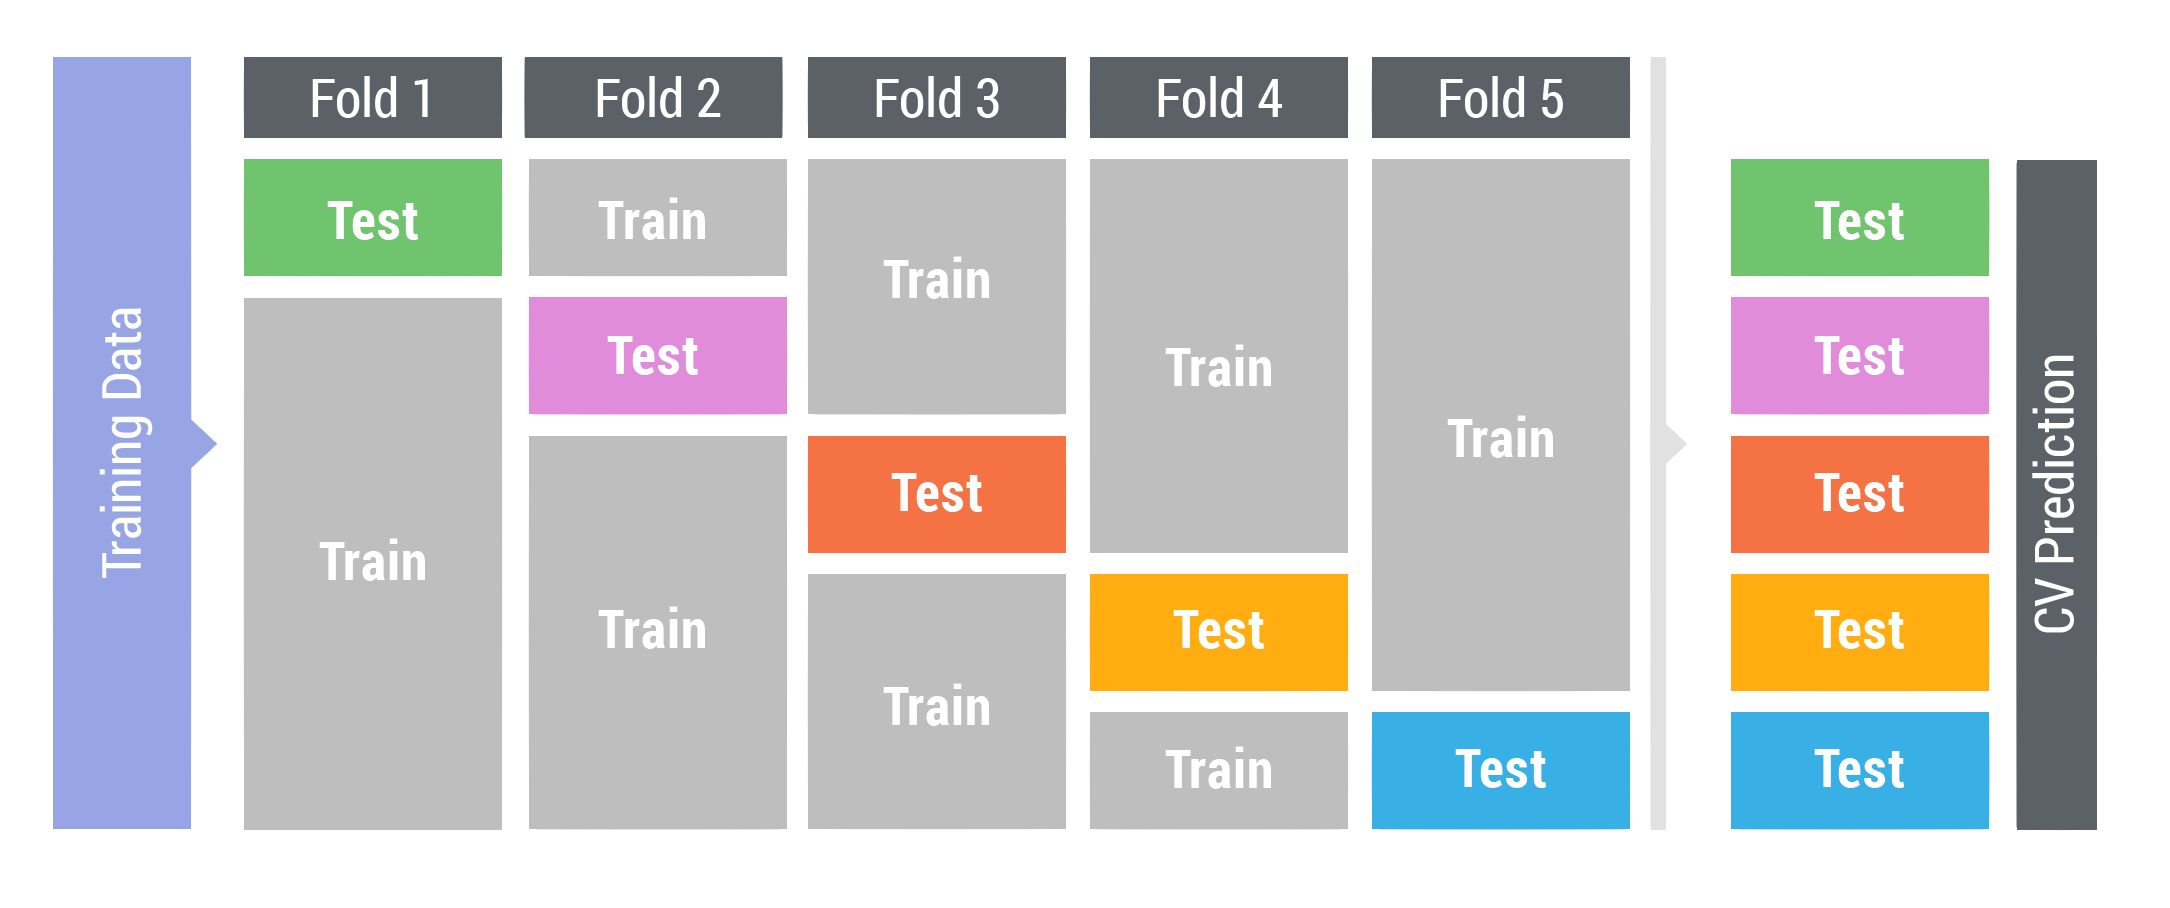
\includegraphics[width=0.5 \textwidth]{cv}
    \caption{5-fold CV.}
\end{figure}

We used stratified 5-fold CV for model validation and ensemble.
As shown in Figure 3, training data were split into 5 folds while the sample size and dropout rate were preserved across the folds.

For validation, each of single and ensemble models was trained 5 times. Each time, 1 fold was held out and the remaining 5 folds were used for training. Then, predictions for the hold-out folds were combined and formed the model's CV prediction. CV predictions were used as inputs for ensemble model training as well as the model's CV score calculation.

For test, each of single and ensemble models was retrained with whole training data. Then predictions for test data were used as inputs for ensemble prediction as well as for submission. 

\subsection{Multi-Stage Ensemble}

\begin{figure}[!h]
  \centering
    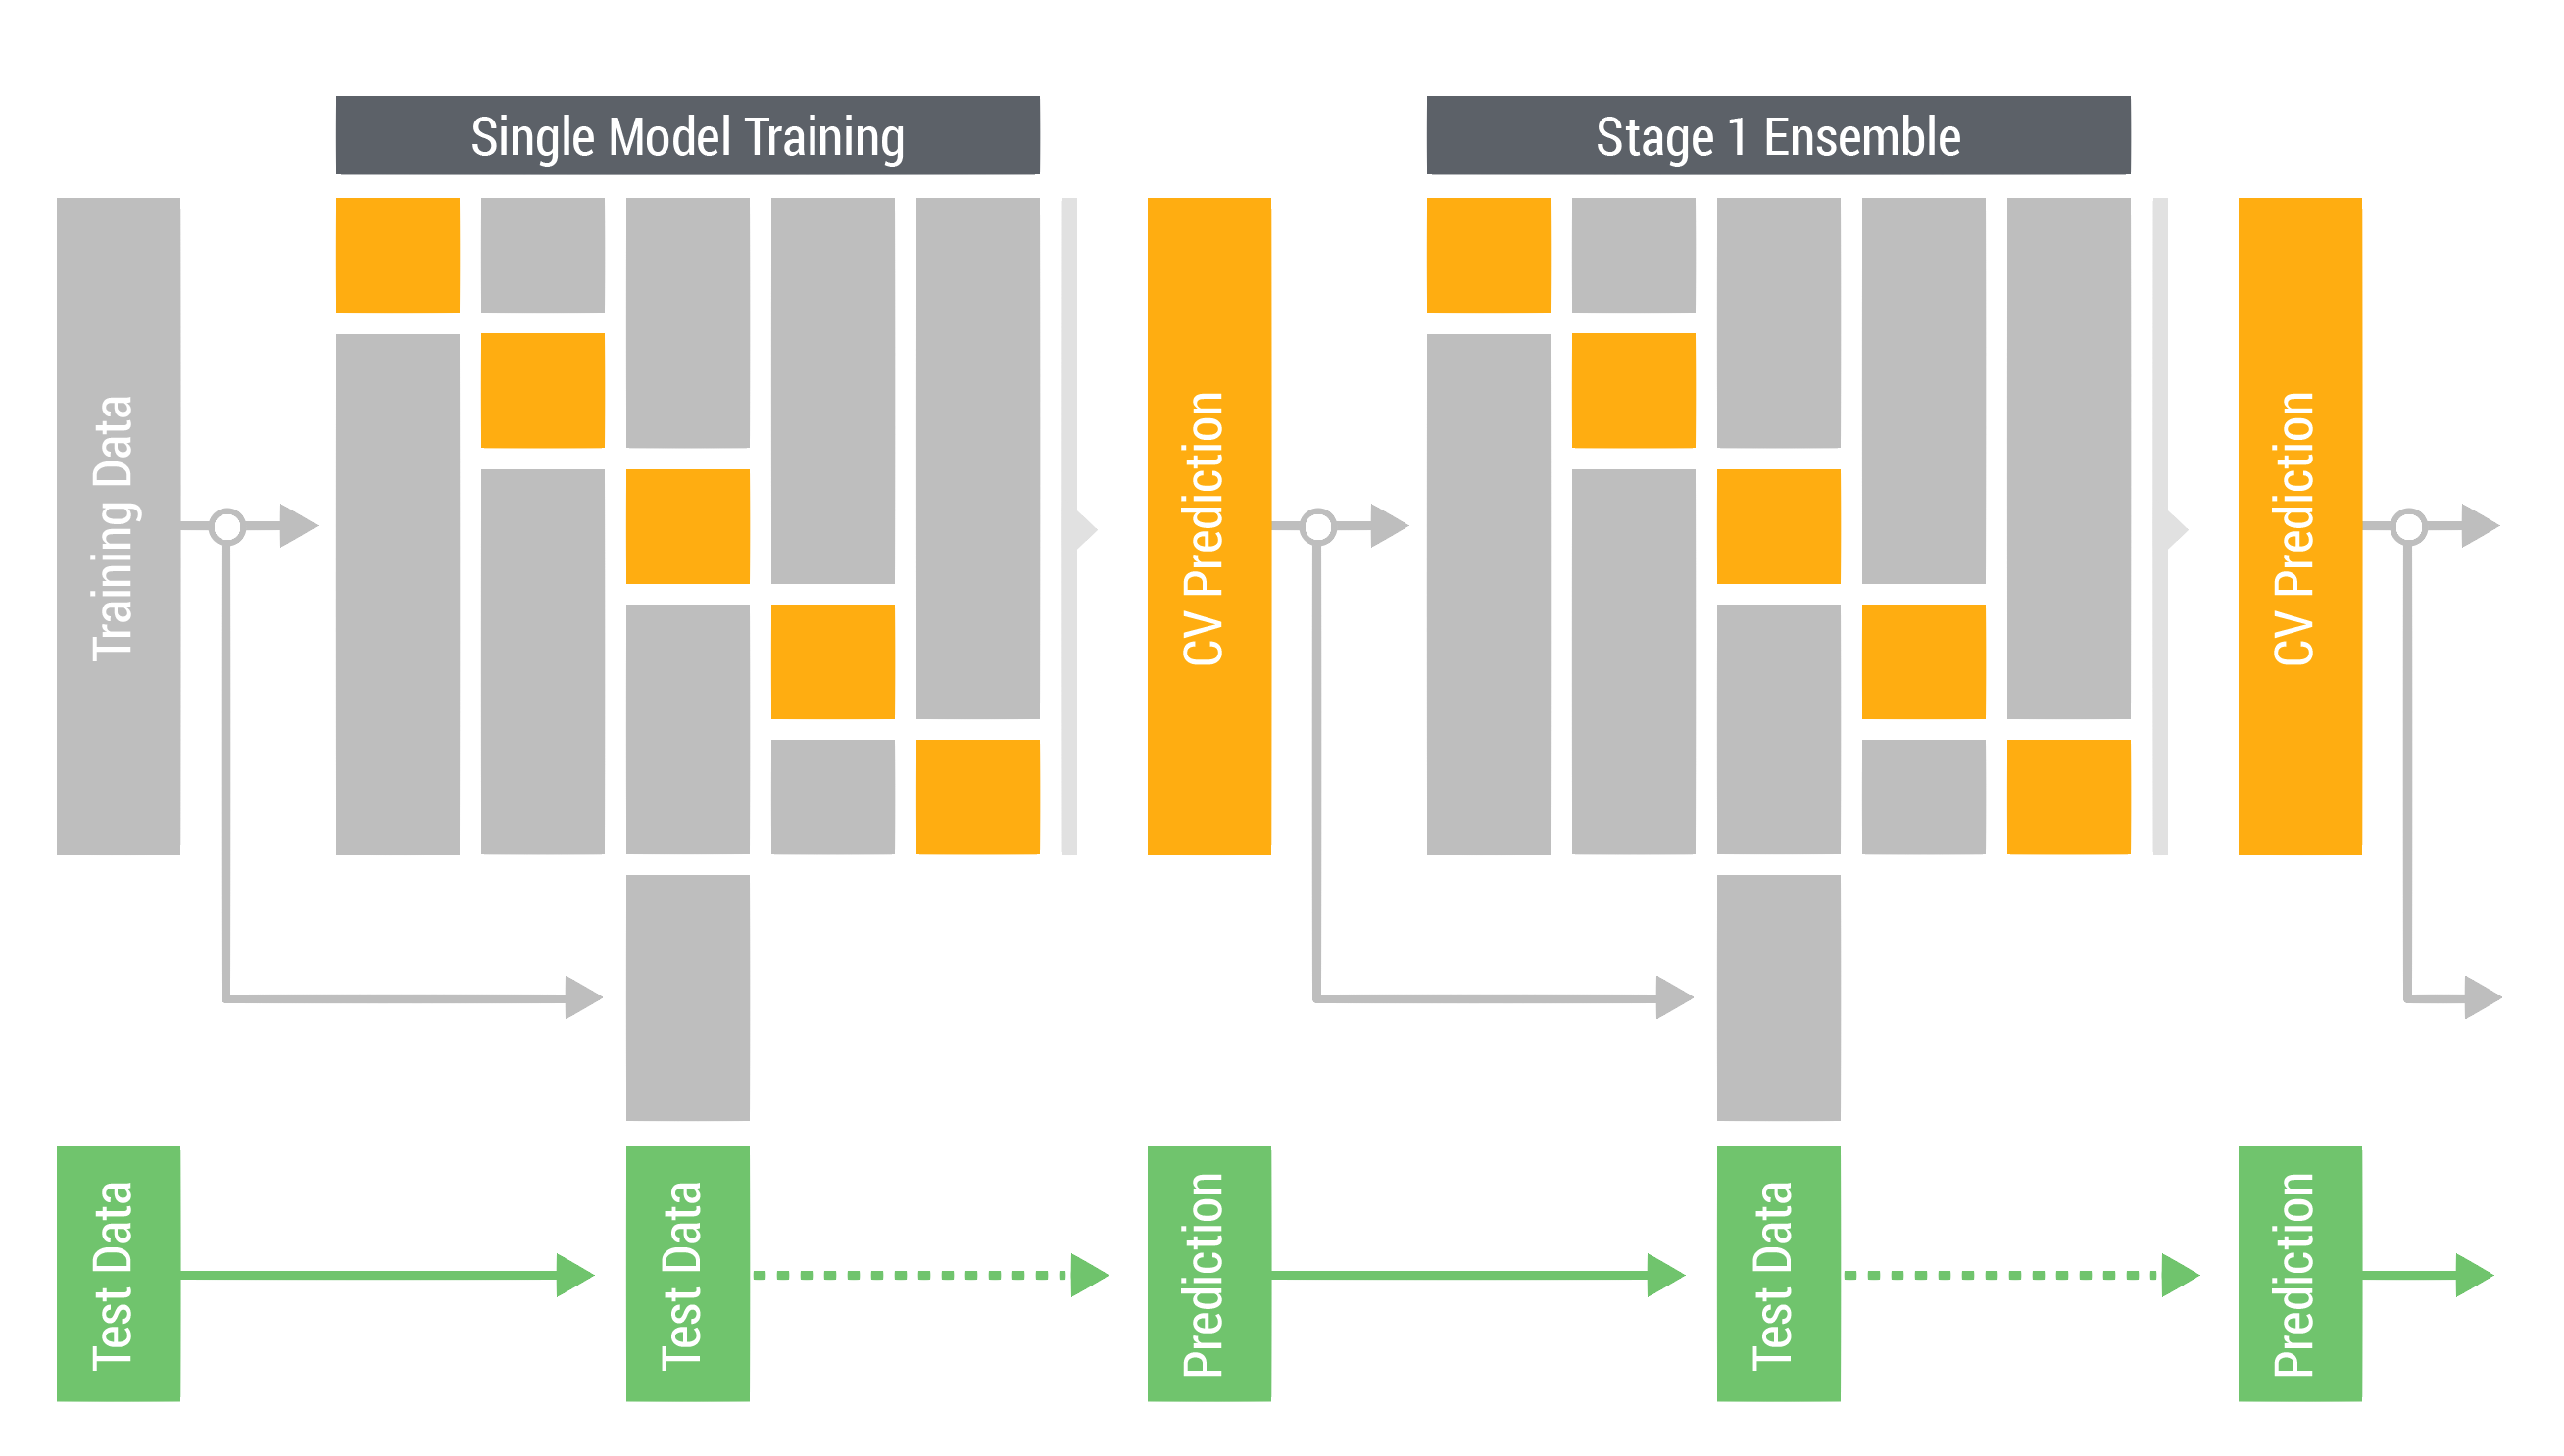
\includegraphics[width=0.5 \textwidth]{cv_ensemble}
      \caption{5-fold CV stacked generalization ensemble.}
\end{figure}

We used the multi-stage ensemble with stacked generalization \cite{wolpert1992stacked, ting1999issues} to blend predictions of various models.  At each stage, we train ensemble models with 5-fold CV, and use the CV and test predictions of models in the previous stage as inputs.  Then, we pass the CV and test predictions of the ensemble models to the next stage as inputs.  Figure 4 illustrates the process of multi-stage ensemble with 5-fold CV stacked generalization.

We stopped adding an additional ensemble stage when we saw no improvement in CV.
\section{Final Solution}
Our final solution is a stage-3 ensemble model trained with the multi-stage ensemble method described in Section 4.2 as follows:
\begin{itemize}
  \setlength\itemsep{0em}
  \item \textbf{Single Model Training}: First, we trained 64 single models with the 8 different algorithms and different subsets of 7 feature sets and DAE features.  Out of 64 models, there were 26 GBM, 14 NN, 12 FM, 6 LR, 2 KRR, 2 ET, 1 RF, and 1 KNN models.  Some of single models used RF feature selection, where we trained an RF model and selected features with high variable importances.
  \item \textbf{Stage-1 Ensemble}: Second, we trained 15 stage-1 ensemble models with different subsets of CV predictions of 64 single models.  Out of 15 models, there were 7 GBM, 4 NN, 2 LR, 1 FM, and 1 ET models.  Some of stage-1 ensemble models used rank orders between single models as additional inputs.  
  \item \textbf{Stage-2 Ensemble}: Third, we trained 2 stage-1 ensemble models with different subsets of CV predictions of 15 stage-1 ensemble models.  We used a LR with stepwise greedy forward selection and a GBM.
  \item \textbf{Stage-3 Ensemble}: Lastly, we trained a stage-3 ensemble model with CV predictions of all models.  We used LR with stepwise greedy forward selection, and it selected 5 models out of total 81 models: 1 stage-2 ensemble models, 3 stage-1 ensemble models and 1 single model.  Table 3 shows the list of models selected by the final stage-3 ensemble model.
\end{itemize}

Figure 6 shows the end-to-end pipeline for the final solution.  Details of the single and ensemble models trained are available in Table A3 and A4 in Appendix.

Our final solution achieved AUC scores of 0.90918 and 0.90744 on the public and private leaderboards respectively, and put us to the 1st place out of 821 teams.

At KDD Cup 2015, we made some observations as follows:
\begin{itemize}
\setlength\itemsep{0em}
\item As shown in Figure 5, our CV scores were very consistent with public leaderboard scores.  Therefore we used CV scores to determine (1) whether to add more ensemble stage or not and (2) whether to include a model for ensemble or not.
\item GBM outperformed other algorithms.  Our top 8 single models as well as top 2 stage-1 ensemble models are GBM models.  NN and FM were next best algorithms.  LR with stepwise greedy forward selection worked well in ensemble stages.
\item Biggest performance improvement was from the stage-1 ensemble, and as we added more ensemble stages, we observed diminishing improvements.  The stage-1, -2, and -3 ensembles improved the best CV score by 0.00967, 0.00028, and 0.000226 respectively.  However, it was the improvement from the stage-2 and -3 ensemble that allowed us to finish the 1st.
\end{itemize}

\begin{figure}[t]
  \centering
    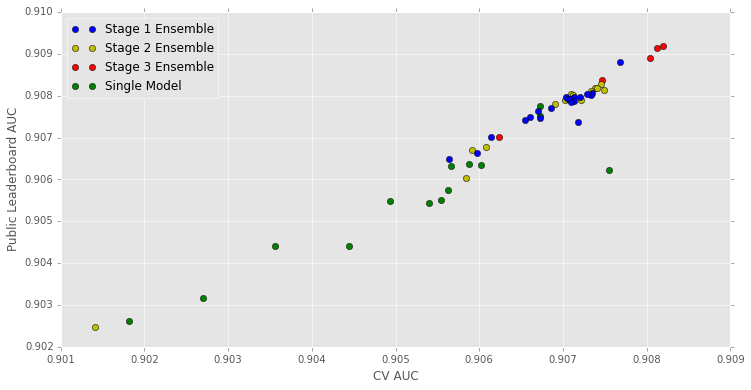
\includegraphics[width=0.5 \textwidth]{cv_lb}
      \caption{CV vs. public leaderboard AUC scores.}
\end{figure}

\begin{figure}[!t]
  \centering
    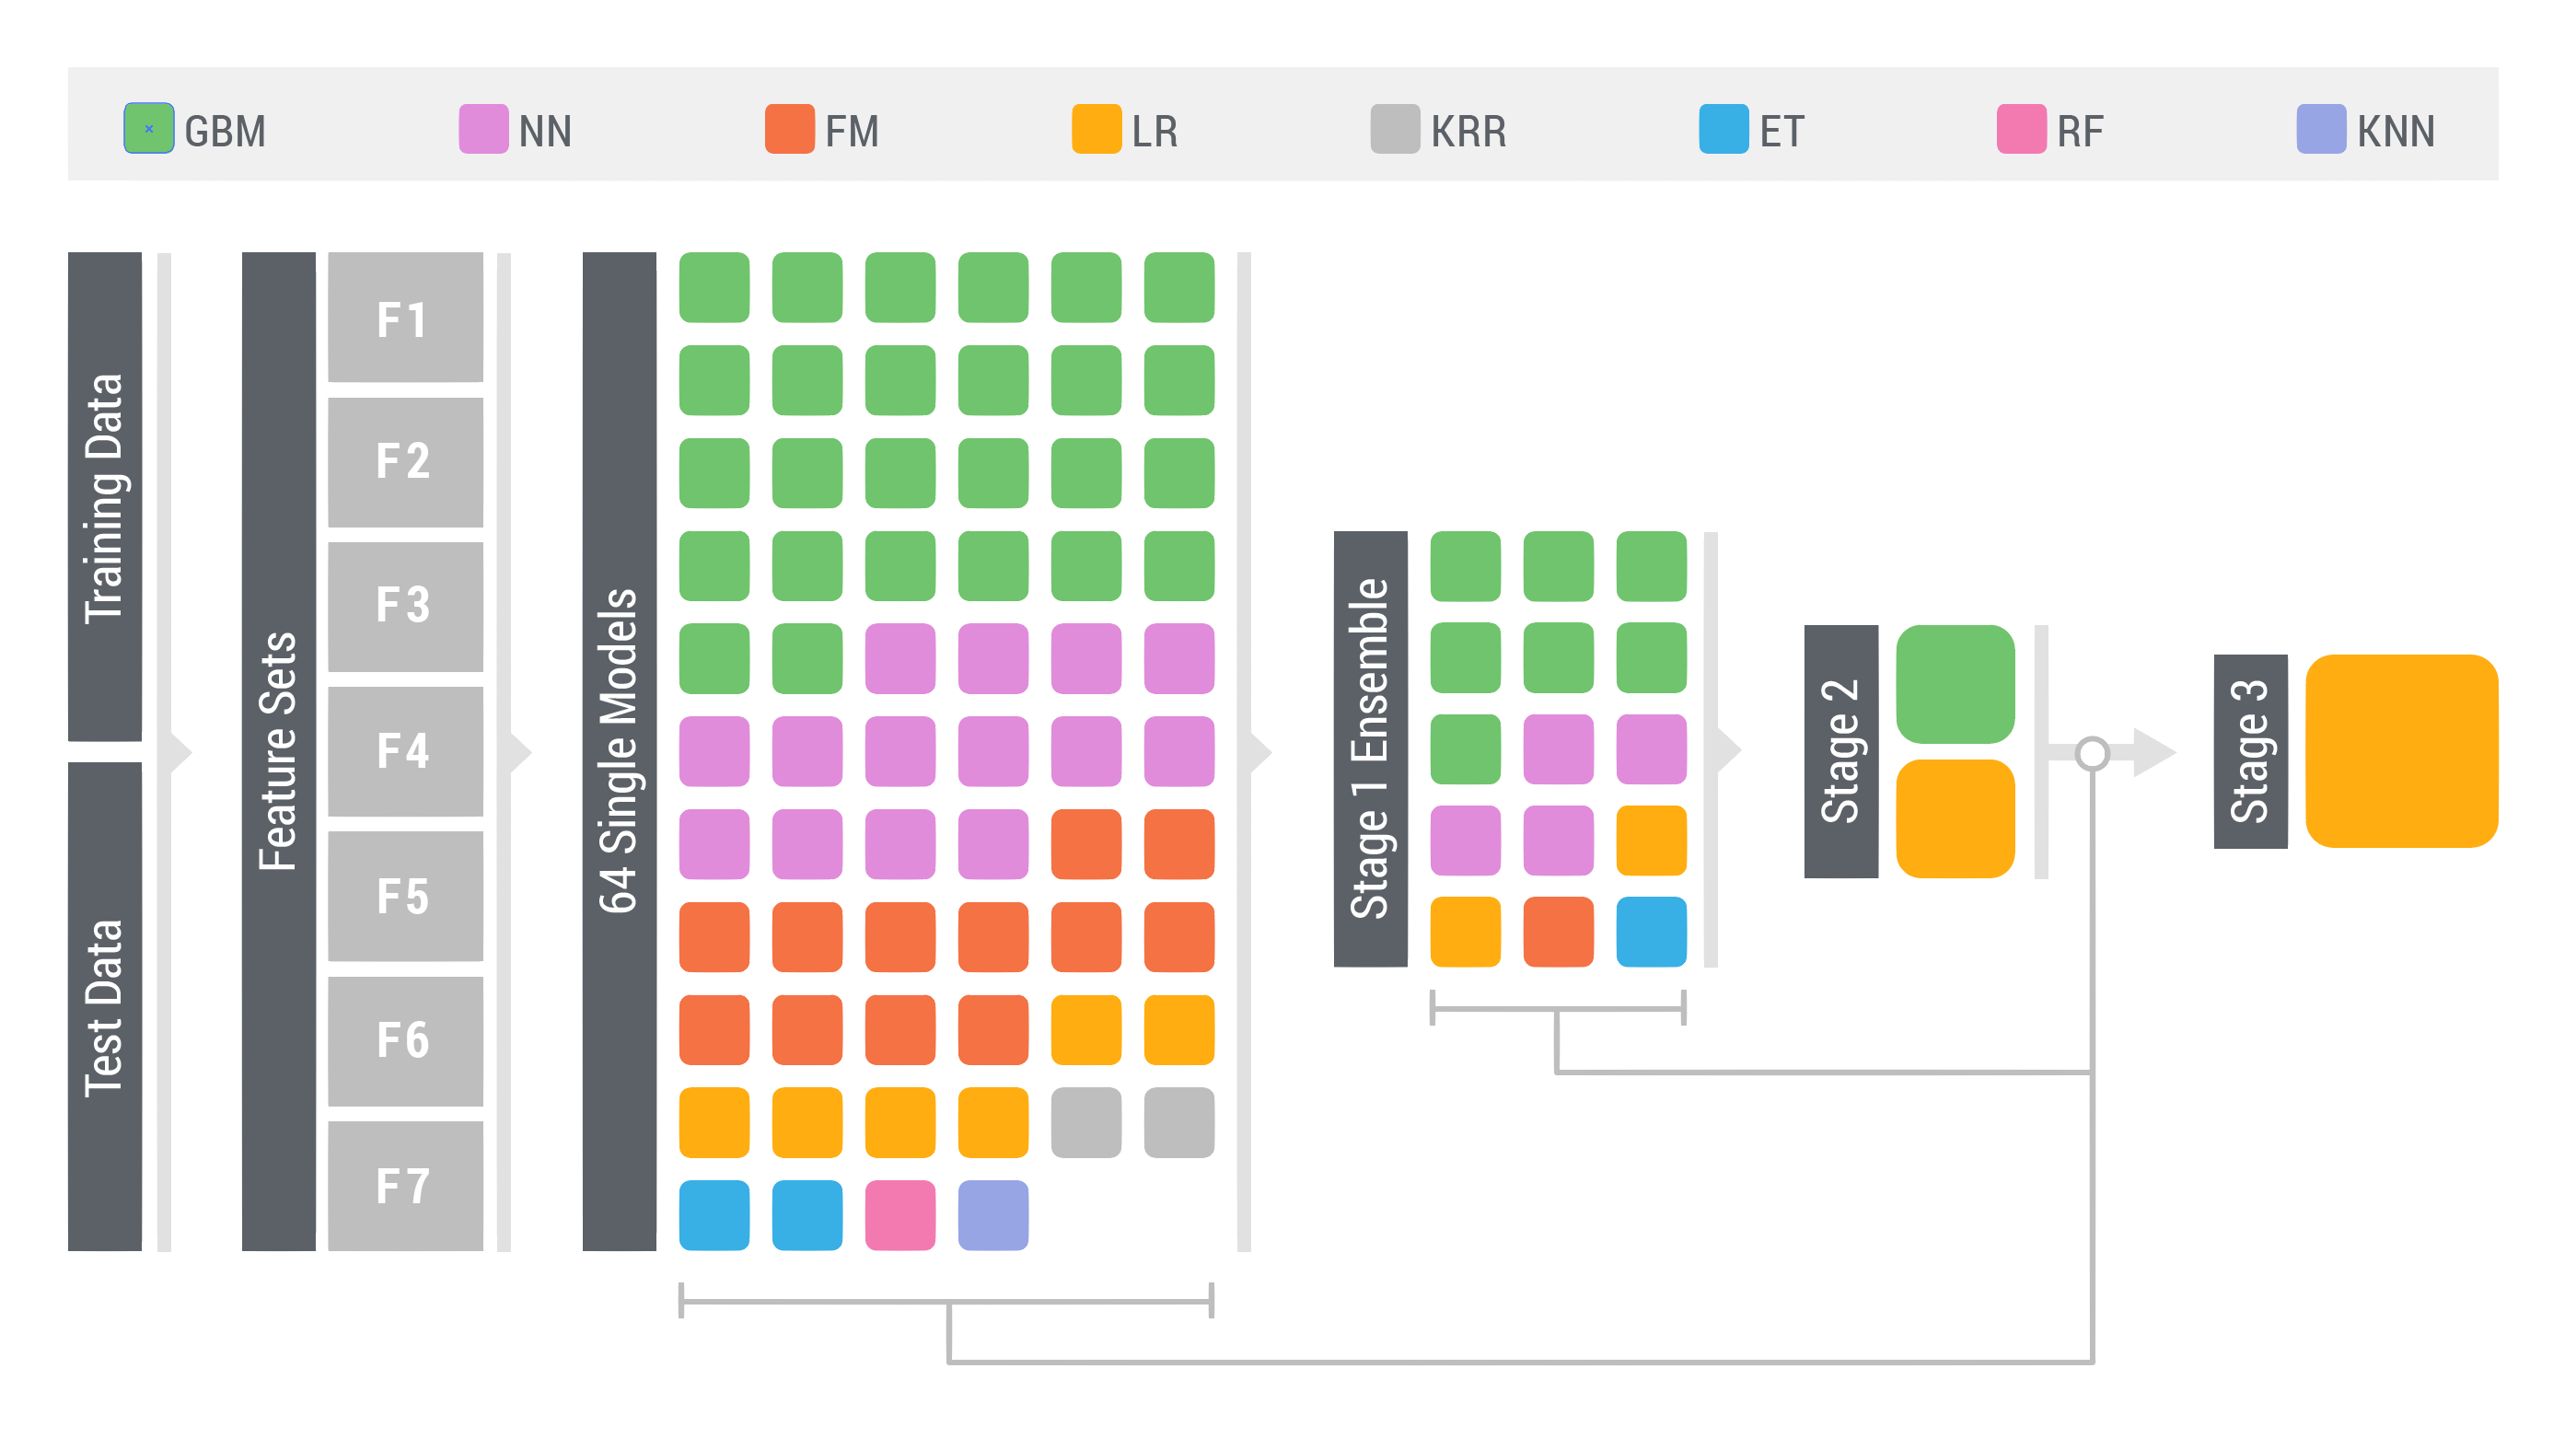
\includegraphics[width=0.5 \textwidth]{ensemble}
      \caption{End-to-end pipeline for the final solution}
\end{figure}

\begin{table}
\begin{center}
	\caption{Models selected in the stage-3 ensemble.}
\begin{tabular}{lllll}
ID 	& Stage 	& Algorithm 	& 5-CV 		& Weight\\ \hline
S1 	& Single	& GBM		& 0.906721 	& 1.1703 \\
E4 	& 1 		& GBM		& 0.907878 	& 1.9626\\
E8 	& 1 		& NN		& 0.907567	& 0.7871\\
E18	& 1		& ET			& 0.906207 	& 0.4580\\
E2	& 2 		& LR			& 0.907968 	& 1.6146\\
\end{tabular}

\label{tb:finalEnsemble}
\end{center}
\end{table}


% An example of a floating figure using the graphicx package.
% Note that \label must occur AFTER (or within) \caption.
% For figures, \caption should occur after the \includegraphics.
% Note that IEEEtran v1.7 and later has special internal code that
% is designed to preserve the operation of \label within \caption
% even when the captionsoff option is in effect. However, because
% of issues like this, it may be the safest practice to put all your
% \label just after \caption rather than within \caption{}.
%
% Reminder: the "draftcls" or "draftclsnofoot", not "draft", class
% option should be used if it is desired that the figures are to be
% displayed while in draft mode.
%
%\begin{figure}[!t]
%\centering
%\includegraphics[width=2.5in]{myfigure}
% where an .eps filename suffix will be assumed under latex, 
% and a .pdf suffix will be assumed for pdflatex; or what has been declared
% via \DeclareGraphicsExtensions.
%\caption{Simulation results for the network.}
%\label{fig_sim}
%\end{figure}

% Note that the IEEE typically puts floats only at the top, even when this
% results in a large percentage of a column being occupied by floats.


% An example of a double column floating figure using two subfigures.
% (The subfig.sty package must be loaded for this to work.)
% The subfigure \label commands are set within each subfloat command,
% and the \label for the overall figure must come after \caption.
% \hfil is used as a separator to get equal spacing.
% Watch out that the combined width of all the subfigures on a 
% line do not exceed the text width or a line break will occur.
%
%\begin{figure*}[!t]
%\centering
%\subfloat[Case I]{\includegraphics[width=2.5in]{box}%
%\label{fig_first_case}}
%\hfil
%\subfloat[Case II]{\includegraphics[width=2.5in]{box}%
%\label{fig_second_case}}
%\caption{Simulation results for the network.}
%\label{fig_sim}
%\end{figure*}
%
% Note that often IEEE papers with subfigures do not employ subfigure
% captions (using the optional argument to \subfloat[]), but instead will
% reference/describe all of them (a), (b), etc., within the main caption.
% Be aware that for subfig.sty to generate the (a), (b), etc., subfigure
% labels, the optional argument to \subfloat must be present. If a
% subcaption is not desired, just leave its contents blank,
% e.g., \subfloat[].


% An example of a floating table. Note that, for IEEE style tables, the
% \caption command should come BEFORE the table and, given that table
% captions serve much like titles, are usually capitalized except for words
% such as a, an, and, as, at, but, by, for, in, nor, of, on, or, the, to
% and up, which are usually not capitalized unless they are the first or
% last word of the caption. Table text will default to \footnotesize as
% the IEEE normally uses this smaller font for tables.
% The \label must come after \caption as always.
%
%\begin{table}[!t]
%% increase table row spacing, adjust to taste
%\renewcommand{\arraystretch}{1.3}
% if using array.sty, it might be a good idea to tweak the value of
% \extrarowheight as needed to properly center the text within the cells
%\caption{An Example of a Table}
%\label{table_example}
%\centering
%% Some packages, such as MDW tools, offer better commands for making tables
%% than the plain LaTeX2e tabular which is used here.
%\begin{tabular}{|c||c|}
%\hline
%One & Two\\
%\hline
%Three & Four\\
%\hline
%\end{tabular}
%\end{table}


% Note that the IEEE does not put floats in the very first column
% - or typically anywhere on the first page for that matter. Also,
% in-text middle ("here") positioning is typically not used, but it
% is allowed and encouraged for Computer Society conferences (but
% not Computer Society journals). Most IEEE journals/conferences use
% top floats exclusively. 
% Note that, LaTeX2e, unlike IEEE journals/conferences, places
% footnotes above bottom floats. This can be corrected via the
% \fnbelowfloat command of the stfloats package.




\section{Conclusions}
Our final AUC score of 0.90918 results from a complex pipeline from raw data to final score.
Every part of that pipe needs to be (sub-)optimal implemented by our team to get the best score at the end.
The first part ``feature design'' is the most important one and needs expertise, experience and of course a bit luck to capture all signals in the data.


% conference papers do not normally have an appendix


% use section* for acknowledgment
\section*{Acknowledgment}


The authors would like to thank...





% trigger a \newpage just before the given reference
% number - used to balance the columns on the last page
% adjust value as needed - may need to be readjusted if
% the document is modified later
%\IEEEtriggeratref{8}
% The "triggered" command can be changed if desired:
%\IEEEtriggercmd{\enlargethispage{-5in}}

% references section

% can use a bibliography generated by BibTeX as a .bbl file
% BibTeX documentation can be easily obtained at:
% http://mirror.ctan.org/biblio/bibtex/contrib/doc/
% The IEEEtran BibTeX style support page is at:
% http://www.michaelshell.org/tex/ieeetran/bibtex/
%\bibliographystyle{IEEEtran}
% argument is your BibTeX string definitions and bibliography database(s)
%\bibliography{IEEEabrv,../bib/paper}
%
% <OR> manually copy in the resultant .bbl file
% set second argument of \begin to the number of references
% (used to reserve space for the reference number labels box)
\bibliographystyle{IEEEtran}
\bibliography{icdm_ice}


% that's all folks
\end{document}


